\section{Simulation Results} \label{sec:results}
The simulation environment used was Gazebo \cite{gazebo}, the standard simulation tool for ROS-based projects. In addition to providing a 3D visualization of the robot and environment, Gazebo also simulates the physics, sensory input, and odometry for the robot. All tests were run under Ubuntu 18.04 on a machine with a \SI{3.6}{GHz} Intel Core i7-7700 processor, an NVidia GeForce GTX 1070 video card, and \SI{16}{GB} of memory.

Two types of test scenarios were created. The first was a set of general purpose scenarios in which the robot was tasked with painting lengths of walls at varying locations and orientations throughout a \SI{10}{\meter}$\times$\SI{7}{\meter} room a single color (see figure \ref{fig:paintbot_room}). These tests were designed to collect data about the speed and accuracy of the robot's actions. The second type of test was a set of scenarios with scenes that contained varying numbers of paint colors and wall sections. These tests were designed to evaluate the ability of the robot to plan for tasks of varying complexity.
\begin{figure}
    \centering
    \begin{subfigure}{0.45\linewidth}
        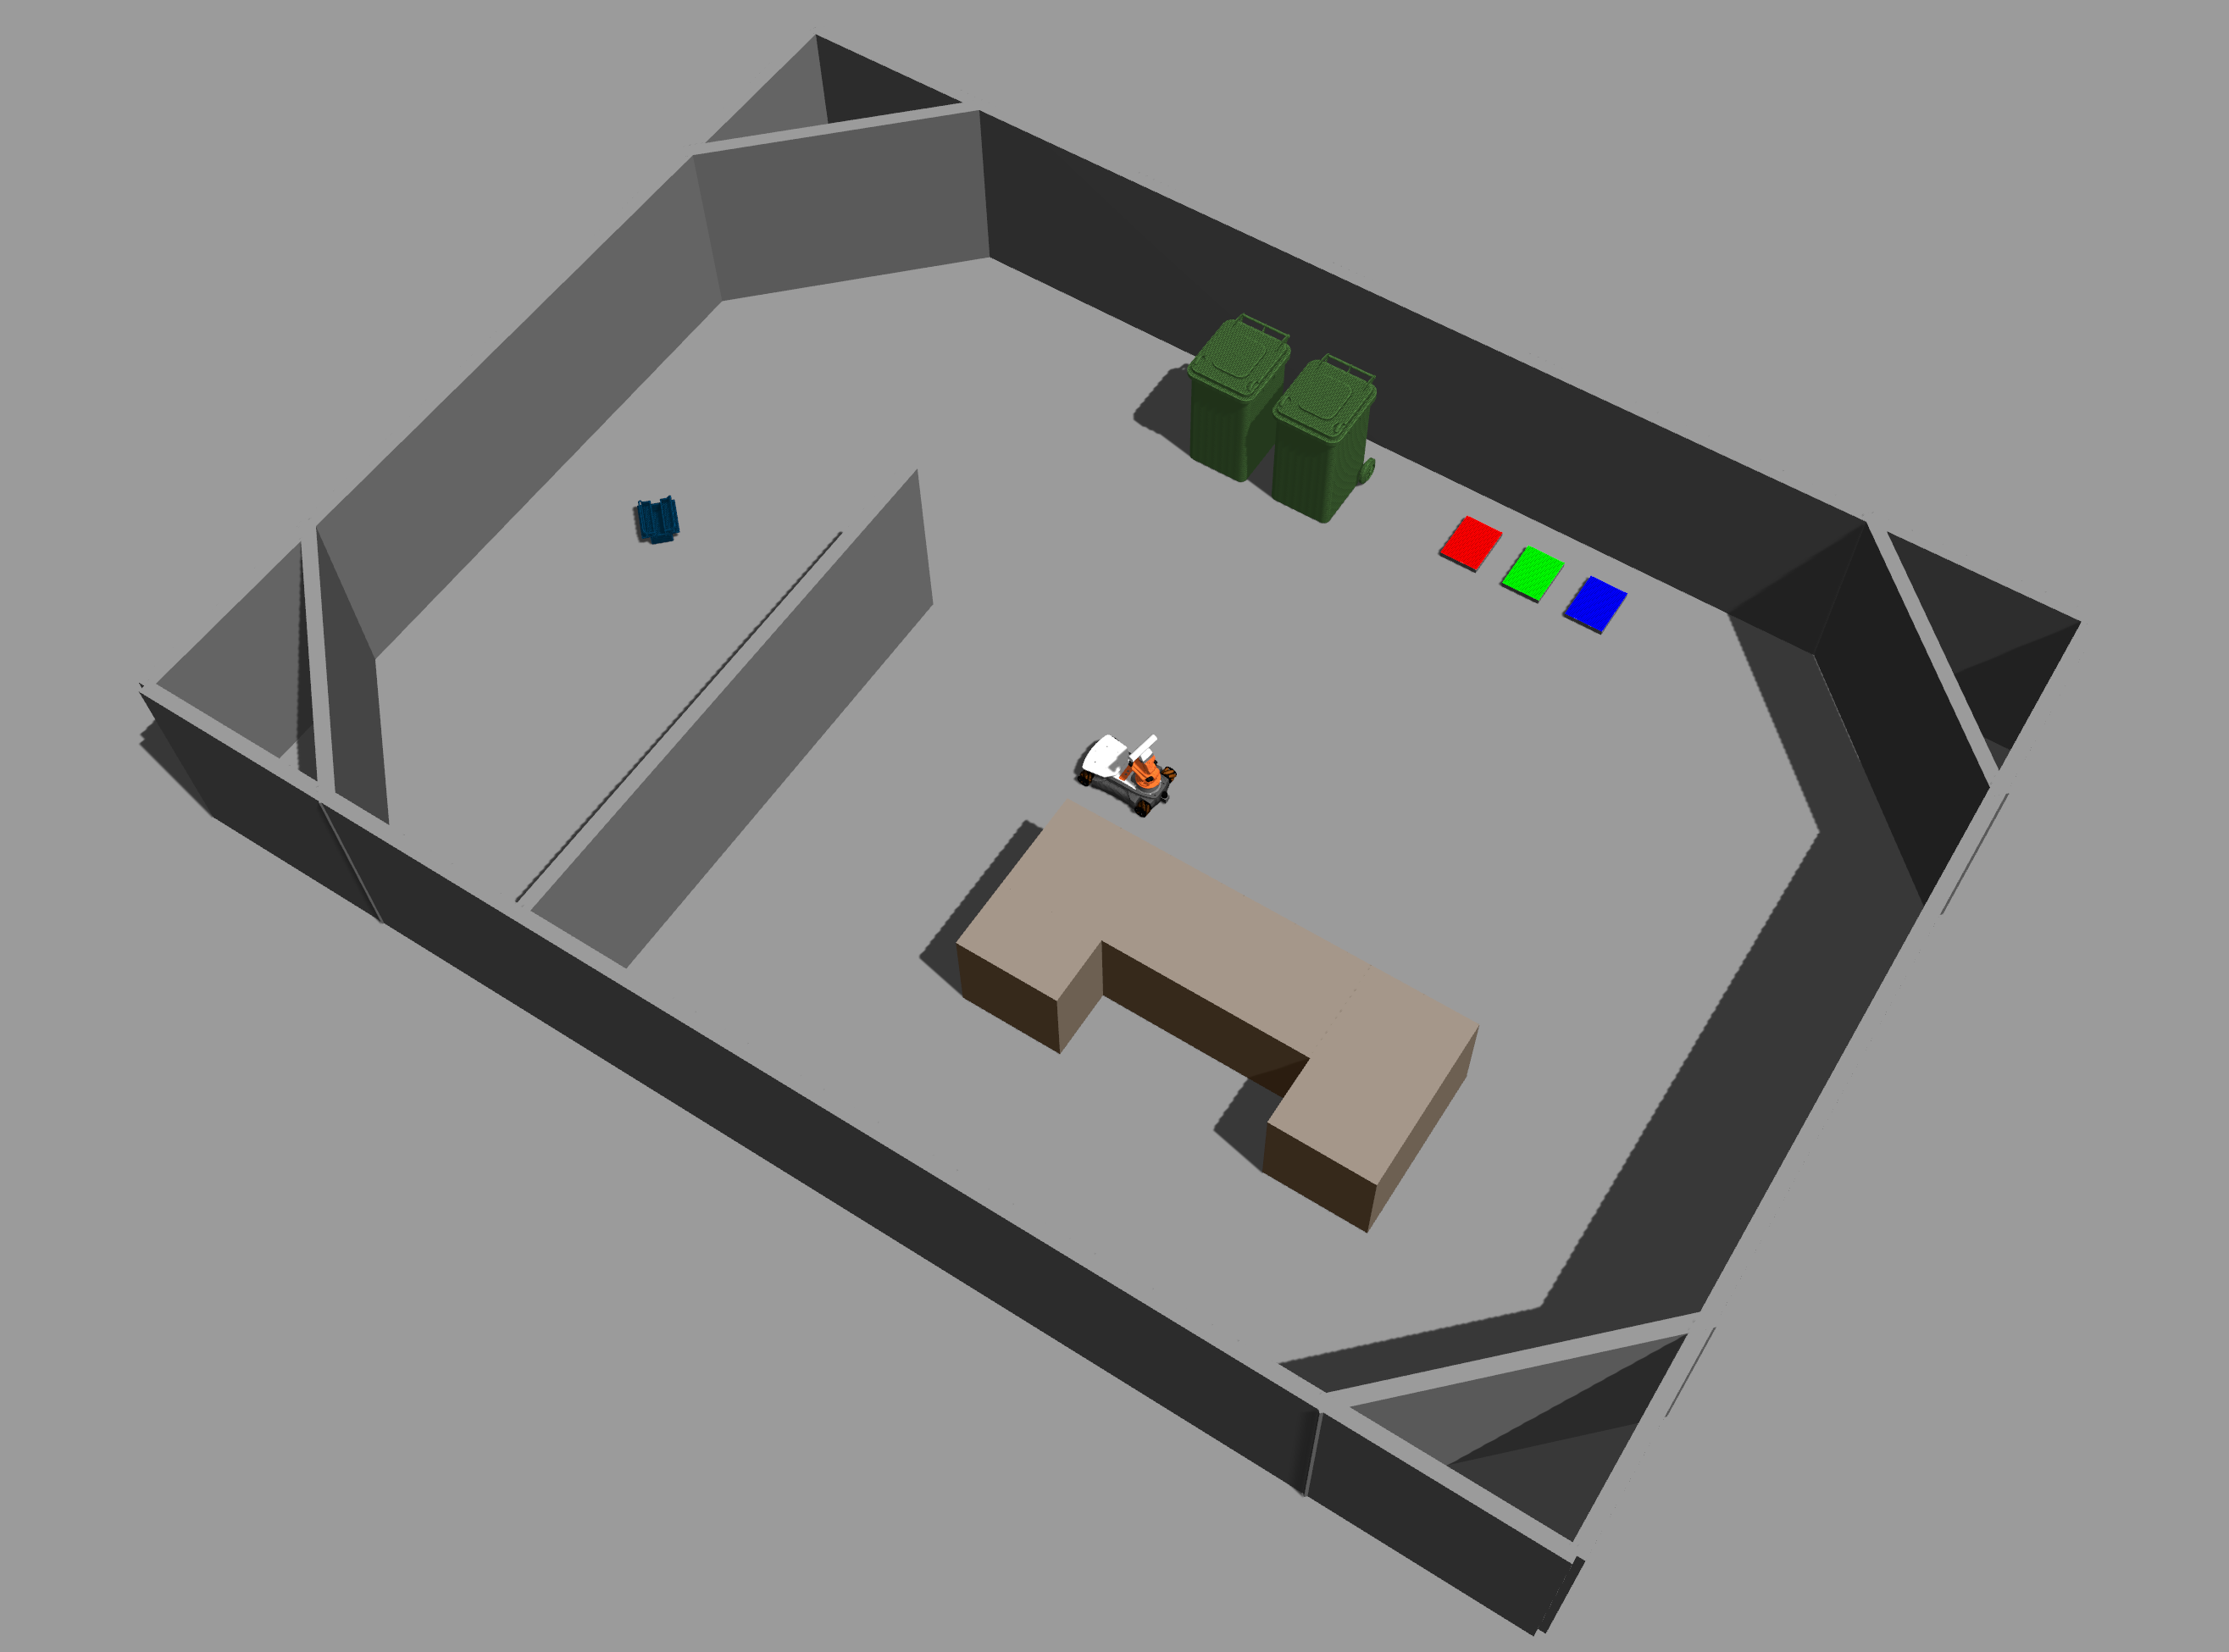
\includegraphics[width=\linewidth]{images/sim_room.png}
        \caption{Simulated room}
        \label{fig:paintbot_room}
    \end{subfigure}
    \hfill
    \begin{subfigure}{0.45\linewidth}
        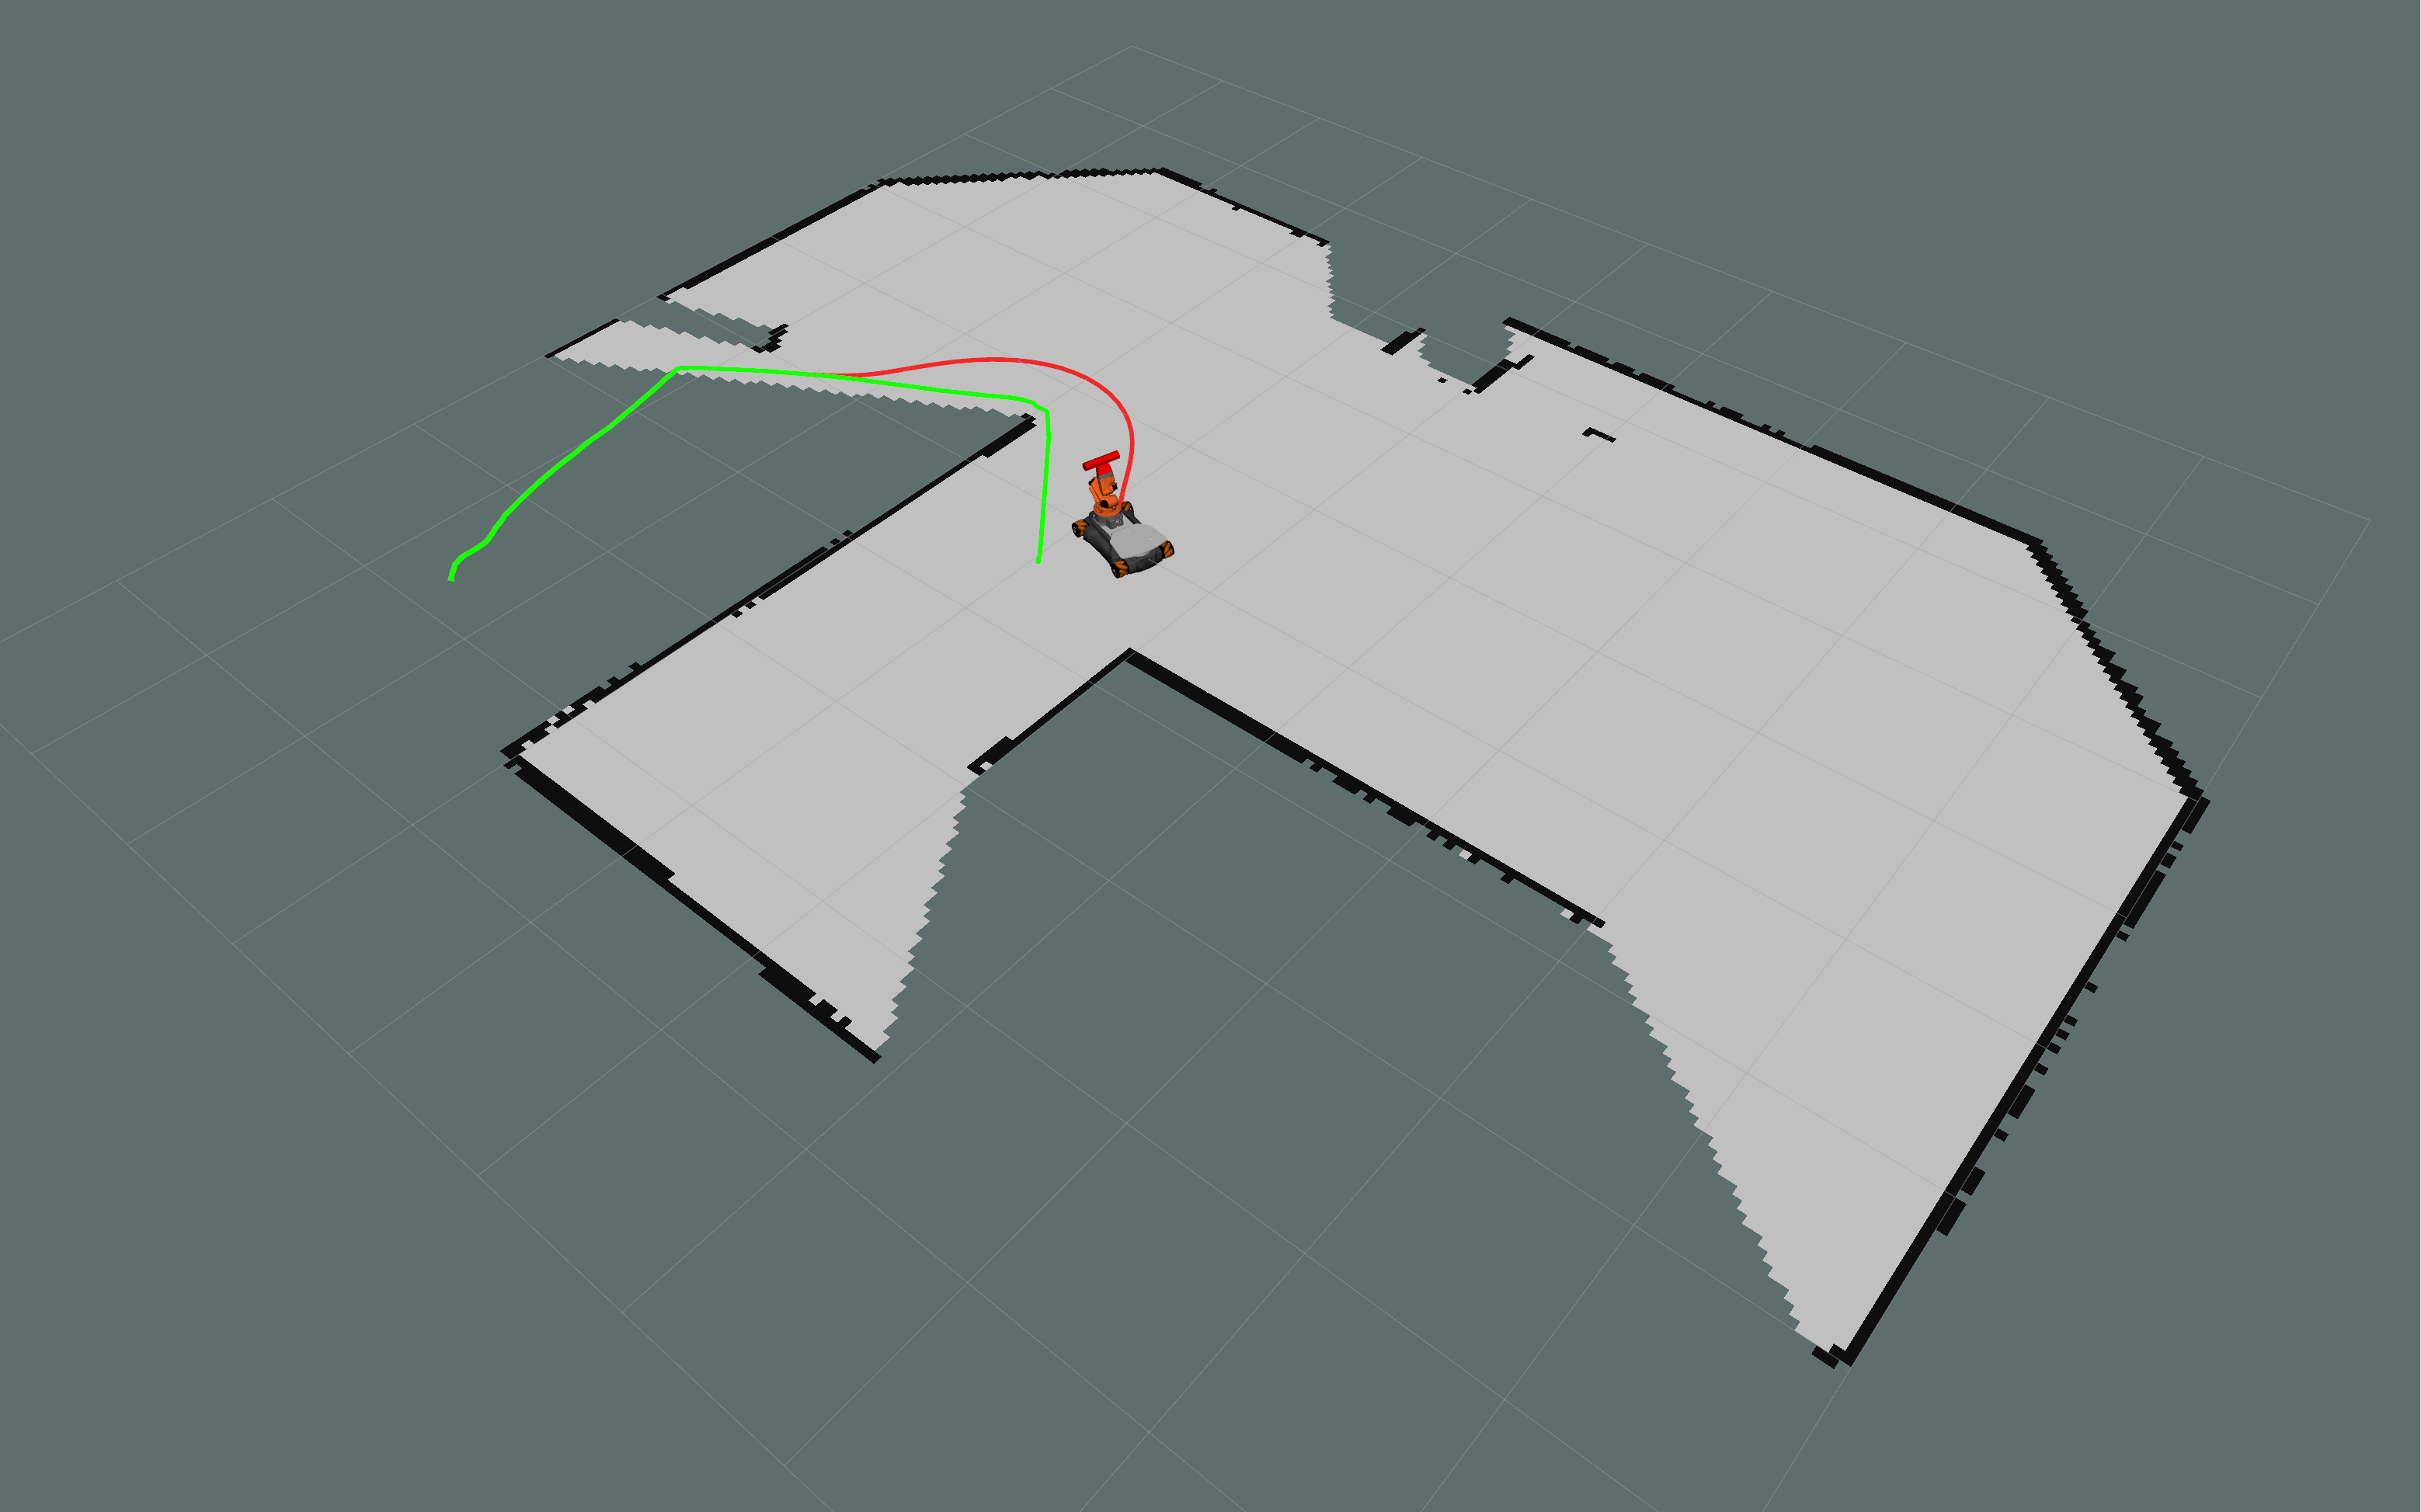
\includegraphics[width=\linewidth]{images/rviz_nav.png}
        \caption{SLAM visualization}
        \label{fig:paintbot_nav}
    \end{subfigure}
    \caption{\ref{fig:paintbot_room} shows the room used during simulations containing three paint trays along one wall, walls with varying orientations, and a few obstacles. \ref{fig:paintbot_nav} shows a visualization of the robot's map of the room and path planning. The green and red lines are the global and local TEB trajectories, respectively.}
    \label{fig:paintbot_runtime}
\end{figure}

The skills and scenes were designed with the intent that the robot performs the following sequence of tasks for each wall section:
\begin{enumerate}
    \item Navigate to the paint tray containing the color required by the wall section.
    \item Load paint from the paint tray onto the roller at the end of the manipulator arm. The arm makes three passes back and forth (for a total of six motions) to ensure the roller is coated.
    \item Navigate to the wall section.
    \item Apply paint to the wall section. The arm makes three passes up and down (for a total of six motions) to ensure the paint is fully applied.
\end{enumerate}
It is likely that the set of skills required in a practical setting would differ from what is presented here. For example, the robot may be equipped with a reservoir of paint and may not need to return to a paint tray between applications. However, The load+apply loop was created to showcase interaction between skills and to increase planning complexity. In this case, the planner must be able to recognize that the arm no longer has enough paint to paint the next wall section and must first perform the LoadPaint skill before continuing.

\subsection{General Test Results}
Each general test scenario specified one length of wall to be painted a single color. The length of wall was approximately \SI{1}{\meter} long, composed of $5-7$ wall sections, and was oriented in one of the \ang{45} increments in the range [\ang{0}, \ang{360}). The walls were selected such that the robot would have to navigate around the various obstacles in the room as it travelled between the paint tray and the wall. Each scenario was simulated $5$ times for a total of $40$ simulations ($8$ angles $\times$ $5$ runs).

\begin{figure}
    \centering
    \resizebox{0.90\linewidth}{!}{
        \begin{tikzpicture}
            \begin{axis}
            [
                xlabel={Duration (s)},
                ytick={1,2,3,4},
                yticklabels={ApplyPaintPrim, ArmToZeroPrim, LoadPaintPrim, NavToLocPrim}
            ]
            % ApplyPaintPrim
            \addplot+[
                boxplot prepared={
                    lower whisker=21.8184,
                    lower quartile=22.446975,
                    median=22.92375,
                    upper quartile=24.979375,
                    upper whisker=28.0878
                }
            ] coordinates {};
            % ArmToZeroPrim
            \addplot+[
                boxplot prepared={
                    lower whisker=0.0006,
                    lower quartile=4.49445,
                    median=4.5282,
                    upper quartile=5.6854,
                    upper whisker=5.7979
                }
            ] coordinates {};
            % LoadPaintPrim
            \addplot+[
                    boxplot prepared={
                    lower whisker=19.6744,
                    lower quartile=21.3819,
                    median=22.1672,
                    upper quartile=23.133,
                    upper whisker=27.5227
                }
            ] coordinates {};
            % NavToLocPrim
            \addplot+[
                    boxplot prepared={
                    lower whisker=7.1589,
                    lower quartile=17.8408,
                    median=23.3068,
                    upper quartile=48.4461,
                    upper whisker=48.4461,
                    %   upper whisker=398.6586
                }
            ] coordinates {};
            \end{axis}
        \end{tikzpicture}
    }
    \caption{A box plot of the execution time of each primitive skill. The upper whisker of the NavigateToLocationPrimitive plot has been truncated for visualization purposes -- this skill had a maximum recorded duration of \SI{398.6586}{\second}. The plot has been otherwise unaltered.}
    \label{fig:prim_time}
\end{figure}

Figure \ref{fig:prim_time} shows the execution time of each of the primitive skills across all simulations. The skills involving arm motion -- ApplyPaintPrimitive, ArmToZeroPrimitive, and LoadPaintPrimitive -- all show fairly consistent timings. This is due to the fact that, as they are currently designed, these motions are highly controlled and predictable. The ArmToZeroPrimitive skill simply returns the arm to a pre-defined position and, predictably, shows the lowest variation. The minimum recorded time for this skill is \SI{0.0006}{\second}, which is likely an erroneous value and may be considered an outlier. The execution times of the ApplyPaintPrimitive and LoadPaintPrimitive skills are very similar, as these skills cause the arm to perform essentially the same basic motion differing primarily in angle. Variation in the arm skill execution times is driven largely by the planning time of the MoveIt package.

The NavigateToLocationPrimitive skill exhibits a much wider range of execution time than the arm-based skills. Some variation is expected since the distance the robot must travel between locations and the obstacles it must navigate around will vary greatly and be unpredictable. The upper end of times taken by the NavigateToLocationPrimitive skill is noteworthy, however. As seen in figure \ref{fig:paintbot_room}, the room used during the simulations is not overly large and the obstacles are not overly complicated and thus does not warrant such high navigation times. These times are the result of several navigation problems that were observed.

First, the robot would occasionally take highly circuitous paths to arrive at its destination. In some instances, this was due to the fact that the TEB algorithm would plan routes through obstacles that had not yet been observed by the laser rangefinder. In such a scenario, the plan would have to be adjusted online to account for these obstacles as they came into the laser's field of view. In other instances, the TEB algorithm would fail to plan a shorter, more direct path and would instead settle on a longer path for unknown reasons. Second, the TEB algorithm would occasionally generate tight loops in the path near the goal that would cause the robot to make in-place or nearly-in-place rotations. This is likely due to both the curving, ``elastic band'' nature of the paths generated by TEB and the balance in the configuration of the algorithm between holonomic and non-holonomic motion. The last, and most predominant, of these problems were oscillations about the destination. Quite often, the TEB algorithm would generate very short, oscillating paths about the destination that could last upwards of several minutes. Navigations that took longer than approximately \SI{420}{\second} were manually terminated. Ten simulations were manually terminated for this reason. It is possible these oscillations are due to a combination of configured tolerances and SLAM update rate, but more investigation is required to confirm this.

\begin{table}
    \centering
    \begin{tabular}{|l|c c c c|}
        \hline
        & Min & Avg & Std Dev & Max \\
        \hline
        \hline
        $\bar{v}$ (m/s) & 0.0000 & 0.2264 & 0.0819 & 0.3473 \\
        \hline
        $\Delta x$ (m) & 0.0006 & 0.1326 & 0.0621 & 0.2174 \\
        \hline
        $\theta$ (rad) & 0.0016 & 0.0857 & 0.0209 & 0.1051 \\
        \hline
    \end{tabular}
    \caption{Metrics collected during the simulations for the velocity of the robot and the accuracy of its positioning.}
    \label{tbl:nav_metrics}
\end{table}

Table \ref{tbl:nav_metrics} shows the metrics collected about the robot's navigation. $\bar{v}$ is the robot's average velocity during the navigation skill, $\Delta x$ is the distance between the robot's destination and its true position at the completion of the navigation skill, and $\theta$ is the difference between the robot's goal heading and its true heading. The TEB algorithm was configured with a goal distance tolerance of \SI{0.2}{\meter}, a goal heading tolerance of \SI{0.1}{rad}, a maximum forward velocity of \SI{0.4}{\meter/\second}, and a maximum reverse velocity of \SI{0.2}{\meter/\second}. The distance and heading tolerances were selected for being the lowest values with which successful navigation paths were able to be generated a majority of the time.

The robot was able to navigate within the defined tolerances the vast majority of the time, as expressed in table \ref{tbl:nav_metrics}. However, these tolerances are not likely to be acceptable for many construction tasks that require precise positioning. If TEB continues to be used for this robot into the future, further work must be done to determine how to reduce these tolerances. A potential solution that could be made is the addition of a secondary fine-grained navigation skill. This skill would activate after the robot has navigated to within the coarse-grained tolerances of TEB and would make more explicit, finer adjustments to the robot's position. The robot's generally low average velocity during the NavigateToLocationPrimitive skill (approximately $57\%$ of its maximum) is largely due the excess movement resulting from the oscillations and loops discussed earlier.

\subsection{Planning Test Results} \label{sec:results_plan}
Each planning test scenario specified a single length of wall to be painted a number of colors. The wall varied between \SI{1}{m} and \SI{5}{m} in length in \SI{1}{m} increments, resulting in a range of $5-24$ wall sections. The number of colors per scenario varied between $1$ and $3$. The length of wall was divided evenly into segments to match the number of paints and a paint was assigned to each one. The scene was generated using the Scene Generator program discussed in section \ref{sec:interaction}. Each scenario was simulated $5$ times for a total of $75$ simulations ($5$ wall lengths $\times$ $3$ paints $\times$ $5$ runs).

\begin{figure}
    \centering
    \resizebox{0.75\linewidth}{!}{
        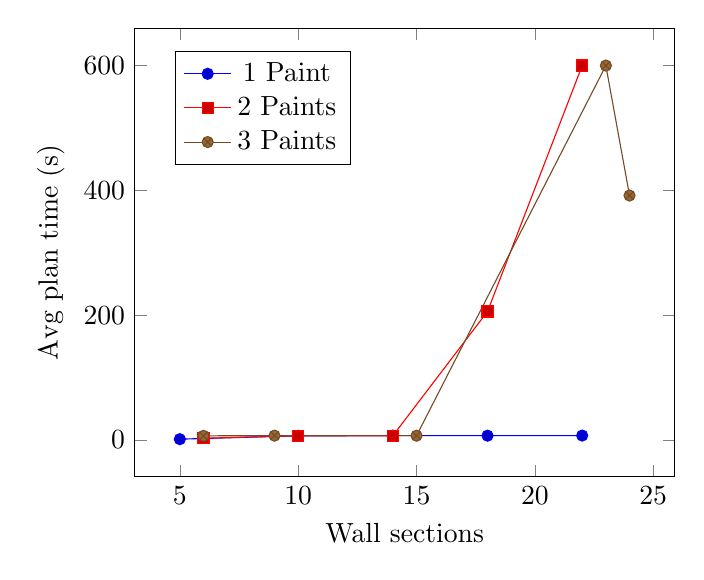
\begin{tikzpicture}
            \begin{axis}
            [
                xlabel={Wall sections},
                ylabel={Avg plan time (s)},
                legend style={at={(0.40,0.95)}}
            ]
            % 1 paint
            \addplot coordinates {(5,1.258) (10,6.705) (14,6.945) (18,6.872) (22,7.051)};
            \addlegendentry{1 Paint}
            % 2 paints
            \addplot coordinates {(6,2.712) (10,6.725) (14,6.760) (18,205.952) (22,600.000)};
            \addlegendentry{2 Paints}
            % 3 paints
            \addplot coordinates {(6,6.595) (9,6.897) (15,6.838) (23,600.000) (24,391.750)};
            \addlegendentry{3 Paints}
            \end{axis}
        \end{tikzpicture}
    }
    \caption{Time taken by the TFD planner to generate plans for a number of paints and an increasing number of wall sections.}
    \label{fig:plan_time}
\end{figure}

Figure \ref{fig:plan_time} shows the planning times for each paint as a function of the number of wall sections. The planning time for a single paint color remained stable at approximately \SI{6.5}{\second}-\SI{7}{\second} across the entire range of wall sections tested for. However, adding additional colors to the scene resulted in erratic and non-obvious changes in the planning time. An extremely sharp increase was observed when the scene contained $2$ or more paints and more than approximately $15$ wall sections. The TFD planner was configured with a time limit of \SI{600}{\second}, after which planning would fail. This happened for two of the scenarios. Curiously, The scenario containing $3$ paints and $24$ wall sections consistently required less planning time than the two less complex scenarios that failed. I have yet to determine the reason for this. 

The times for the $2$ and $3$ paint scenarios are generally too high for practical use and will need to be addressed in the future. The $1$ paint times are adequate for operation inside of a relatively static environment, such as an off-hours construction site where the basic conditions of tasks are unlikely to change. In such a case, online replanning would not be necessary. However, in more dynamic environments where conditions may change rapidly, such as equipment being repositioned by coworkers or new events rendering some tasks impossible, \SI{6.5}{\second}-\SI{7}{\second} may become prohibitively expensive. It should be noted that navigation and obstacle avoidance are performed online and are not part of the task planning process.